\documentclass[11pt]{article}

%%%%%%%%%%%%%%Include Packages%%%%%%%%%%%%%%%%%%%%%%%%%%
\usepackage{xcolor}
\usepackage{mathtools}
\usepackage[a4paper, total={6in, 8in}, margin=1.25in]{geometry}
\usepackage{amsmath}
\usepackage{amssymb}
\usepackage{paralist}
\usepackage{rsfso}
\usepackage{amsthm}
\usepackage{wasysym}
\usepackage[inline]{enumitem}   
\usepackage{hyperref}
\usepackage{tocloft}
\usepackage{titlesec}
\usepackage{colortbl}
\usepackage{wrapfig}
\usepackage{pdfpages}
%%%%%%%%%%%%%%%%%%%%%%%%%%%%%%%%%%%%%%%%%%%%%%%%%%%%%%%%



\begin{document}
\Large \noindent \textbf{Physics 1A Discussion (Week 4)}\\
\normalsize
Department of Physics and Astronomy, UCLA\\
\noindent\rule{8cm}{0.4pt}\\
\noindent The ``Giant Swing" at a county fair consists of a vertical central shaft with a number of horizontal arms attached at its upper end. Each arm supports a seat suspended from a cable that is $5\,$m long. The upper end of a cable is fastened to the arm at a point $3\,$m from the central shaft, as shown in the figure. The cable is hang vertically from the arm when the system is at rest. When the system starts spinning, the cable will make an angle with respect to the vertical axis. 
\begin{center}
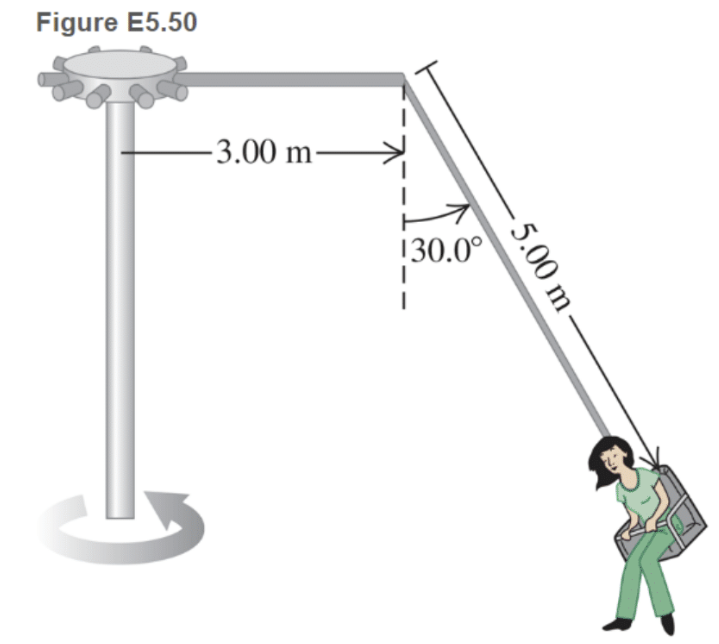
\includegraphics[scale=0.39]{swing.png}
\end{center}

(a) Find the time of one revolution of the swing if the cable supporting a seat makes an angle of $30^\circ$ with the vertical. \\

(b) Does the angle depend on the mass of the passenger for a given rate of revolution?\\


\vfill
\noindent Hint: \color{gray} To solve this problem, start by drawing the free-body diagram of the seat-with-the-passenger. There should be only two forces acting on that, and the sum of the two gives the centripetal force (in what direction? and what magnitude?) such that the seat-with-the-passenger can maintain a circular motion. Now you should be able to determine the tangential speed and such that you can compute the period. 

 
\newpage
\noindent\color{black} Consider two boxes connected by a massless rope. The box $A$ on the table has a weight $45$\,N, and the box $B$ hang by the rope has a weight $25\,$N.

\begin{center}
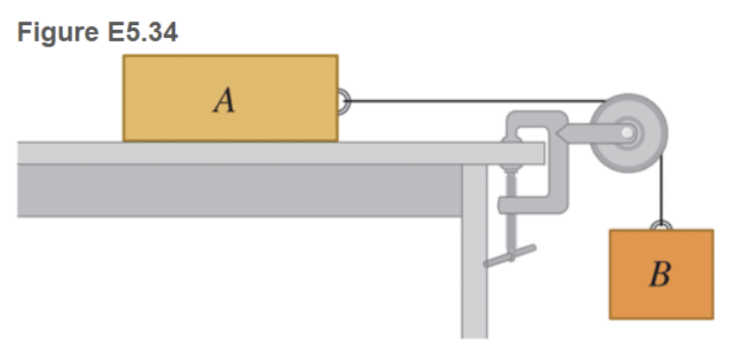
\includegraphics[scale=0.39]{boxes.png}
\end{center}

(a) Once box $B$ is set into downward motion, it descends at a constant speed. Find the coefficient of kinetic friction between box $A$ and the table. \\

(b) Now a cat ($\mathrm{\equiv -.-\equiv}$), of weight $45$\,N, falls asleep on top of box $A$. If box $B$ is set into downward motion again, what would be its acceleration?\\



\vfill
\noindent Hint: \color{gray} To solve this problem, the first step is again drawing free-body diagrams for (1) box $A$ and (2) box $B$. Figure out all forces acting on the boxes symbolically (no need to find them numerically yet). Then write down $F_{\text{net}} = ma$ for each of the two boxes. At this point, we have obtained a system of two equations with two unknowns, and you should be able to solve for the unknowns.\\

\noindent \color{black}BIG HINT: \color{gray} If you are still struggling after reading the first hint, I have done a similar problem in my other discussion sections, you can find its very detailed solution on BruinLearn $\to$ Files $\to$ Discussion worksheets $\to$ 1A$\_$wk4$\_$Q2Hint.pdf \quad :)


\newpage
\color{black}
\textbf{Giant Swing problem:}
Based on the free-body diagram, we have
\begin{align*}
\vec{F} = \left(- F_T \sin(30^\circ) \,,\ F_T\cos(30^\circ)-mg\right)
\end{align*}
for the net force acting on the seat-with-the-passenger, where $m$ is the mass of the seat-with-the-passenger. The system (seat-with-the-passenger) is not accelerating upward or downward, so by $\vec{F} = m\vec{a}$ we must have the vertical component of the net force vanish
\begin{align*}
F_T\cos(30^\circ)-mg = 0\,,
\end{align*}
from which we obtain 
\begin{align*}
F_T = \frac{mg}{\cos(30^\circ)}\,.
\end{align*}
The system undergoes circular motion in a horizontal plane, thus the horizontal component of $\vec{F}$ is the magnitude of the centripetal force, 
\begin{align*}
-F_T \sin(30^\circ) =- \frac{mg }{\cos(30^\circ)}\,\sin(30^\circ) = -\frac{mv^2}{r}\,,
\end{align*}
where $r$ is the radius of the circular path, and the negative signs indicate that these quantities are pointing to the left (at this particular instance indicated on the figure of the problem). From here we can find the tangential speed $v$, 
\begin{align*}
v = \sqrt{rg\tan(30^\circ)}\,,
\end{align*}
and calculate the period,
\begin{align*}
T = \frac{2\pi r}{v} = \frac{2\pi r}{\sqrt{rg \tan(30^\circ)}}\,.
\end{align*}
Now we only need to figure out the radius of the circular motion, which is, according to the geometry in the setup, 
\begin{align*}
r =(3+5\sin(30^\circ))\,\text{m}\,.
\end{align*}
Plug in all the numbers, we find
\begin{align*}
T = 6.19 \, \text{s}\,.
\end{align*}
In our setup above, if the angle $\theta=30^\circ$ were not given (unknown), we can still write down the system of equations from Newton's law,
\begin{align*}
F_T\cos(\theta)+mg = 0\,,\qquad
F_T \sin(\theta) = \frac{mv^2}{r(\theta)}\,.
\end{align*}
Here the radius $r$ depends on the angle $\theta$ based on the geometry in the setup, so we just keep it as a function of $\theta$, denoted as $r(\theta)$. If $T = 2\pi r/v$ is given, we can substitute out $v$ in the system of equations,
\begin{align*}
F_T\cos(\theta) -mg = 0\,,\qquad
F_T\sin(\theta) = \frac{(2\pi\, r(\theta))^2m}{T^2\,r(\theta)}\,.
\end{align*}
Eliminating $F_T$ in the second equation using the first equation we find
\begin{align*}
mg \tan(\theta)= \frac{(2\pi\, r(\theta))^2 m}{T^2 r(\theta)}\,.
\end{align*}
The mass get canceled, 
\begin{align*}
g\tan(\theta) = \frac{2\pi }{T^2}\, r(\theta)\,.
\end{align*}
From this equation, since $r(\theta) = 3+5\sin(\theta)$, it is possible to isolate $\theta$ and write $\theta$ using the other known constants, namely $T$ and $g$. There is not an $m$ in this equation, and thus $\theta$ does not depend on the mass. 

\newpage
\textbf{Two boxes problem:} First we write down the net forces acting on box $A$ and $B$. Box $A$ experiences friction (that has only $x$-component contribution), gravitational and normal forces (only $y$-component contribution), and tension (only $x$-component contribution). In particular, friction has the form
\begin{align*}
\vec{F}_f = (-\mu_k F_N, \, 0)
\end{align*}
where $F_N$ is the magnitude of the gravitational force, and $\mu_k$ is the kinetic friction coefficient. The negative sign indicates that friction points to the left. Now we write
\begin{align*}
\vec{F}_{\text{net, }A} = \vec{F}_f + \vec{F}_T + \vec{F}_N + \vec{F}_g=\left(-\mu_k F_N + F_T\,,\ F_N -m_Ag\right)\,.
\end{align*}
Moreover, since box $A$ is constraint to move on top of the table only, it should have no acceleration on the vertical direction, then the $y$-component of the net force acting on it should vanish, thus 
\begin{align*}
F_N - m_Ag = 0\,,
\end{align*}
which implies $F_N = mg$ and thus 
\begin{align*}
\vec{F}_{\text{net, }A} =\left(-\mu_k m_Ag + F_T\,,\ 0\right)\,.
\end{align*}
Now for box $B$, box $B$ experiences only the force of gravity and tension, both in vertical direction. We can write the net force 
\begin{align*}
\vec{F}_{\text{net, }B} = \left(0\,,\ F_T-m_Bg\right)\,.
\end{align*}
\textbf{The reason that the tension acting on $B$ has the same magnitude as the tension acting on $A$ (but with different directions, vertically up on $B$ and horizontally to the right on $A$) is because the massless rope can have only one tension, it only changes the direction of the tension throughout the rope without changing its magnitude. This is an assumption about a massless rope in this type of problem. Therefore, I have used the same notation $F_T$ in the net force for box $B$ and net force for $A$.} \\

\textbf{When the system starts moving, the two boxes move together, so they should accelerate at the same magnitude (but in different directions, $A$ to the right and $B$ downwards.} Mathematically, this statement can be translated using Newton's second law, 
\begin{align*}
\vec{F}_{\text{net, }A} =\left(-\mu_k m_Ag + F_T\,,\ 0\right) = (m_A a\,,\ 0)\,,\qquad
\vec{F}_{\text{net, }B} = \left(0\,,\ F_T-m_Bg\right) = (0\,,\ -m_B a)\,.
\end{align*} 
Notice that I have use the same acceleration magnitude $a$ for the two boxes. From here we obtain a system of two equations, 
\begin{align*}
\begin{cases}
-\mu_k m_A g +F_T = m_A a\\
F_T - m_B g = -m_B a\end{cases} \,.
\end{align*}
Now we look at the questions. Part (a) states that boxes are moving at constant speed, so $a= 0$ for the two boxes. This allows us to solve for $\mu_k$ in the first equation, 
\begin{align*}
\mu_k = \frac{F_T}{m_Ag}\,,
\end{align*}
where $F_T$ can be obtained from the second equation, 
\begin{align*}
F_T = m_B g\,.
\end{align*}
Thus 
\begin{align*}
\mu_k = \frac{m_B g}{m_A g} = \frac{25}{45} = \frac{5}{9}\,.
\end{align*}

Now for part (b), we again use the system of equations. We have found $\mu_k$ in part (a) so this system now has only two unknowns, $a$ and $F_T$. We can solve for the two unknowns. Also notice that the weight of $A$ is now changed to $m_Ag = 45\text{\,N}+45\,\text{N} = 90\,\text{N}$. Using the second equation, we have
\begin{align*}
F_T = m_Bg - m_B a\,,
\end{align*}
then use the first equation,
\begin{align*}
-\mu_k m_A g + (m_B g - m_B a) =m_A a\,,
\end{align*}
from which we can plug in all numbers to find
\begin{align*}
a = -2.13\,\text{m/s}^2.
\end{align*}
The system is slowing down due to the cat sleeping on box $A$. 
\begin{align*}
\mathrm{\equiv -}&\mathrm{.-\equiv}
\end{align*}


\end{document}


